\section{Data generation}
\subsection{Sampling}
For each of the four cases (NMOS ON/OFF, PMOS ON/OFF) $10{,}000$ samples were drawn, every parameter independently, $V_{DD}$ first:
\begin{center}\small
\begin{tabular}{ll}
\toprule Parameter & Distribution\\\midrule
$V_{DD}$ & uniform, $1\,\mathrm{V}\pm10\%$\\
$V_d$, $V_s$ & uniform, $0$ to $V_{DD}$\\
$W$ & uniform, $1\times L_{\min}$ to $8\times L_{\min}$\\
Temperature & uniform, $-40$ to $125\,^\circ$C\\
vth0, toxe, ndep, u0, xj & uniform, nominal (from the model file) $\pm10\%$, separate NMOS/PMOS values\\
$V_g$, $V_b$ & fixed by the case: NMOS ON $(V_{DD},0)$, NMOS OFF $(0,0)$, PMOS ON $(0,V_{DD})$, PMOS OFF $(V_{DD},V_{DD})$\\
\bottomrule\end{tabular}\end{center}
Each sample is applied to a self-contained single-transistor netlist (model cards inlined with the sampled process parameters, one
voltage source per terminal, one temperature per run). Terminal currents are defined positive \emph{into} the device,
so that $I_d+I_g+I_s+I_b=0$. Simulation of $40{,}000$ samples took about 8.5 minutes; no simulation failed.

\subsection{Data check}
\paragraph{Kirchhoff check.} Table~\ref{tab:kirchhoff} gives the residual $|I_d+I_g+I_s+I_b|$ per case. Where the currents are resolvable
(above about $10^{-15}$\,A) the netlists conserve current to a relative residual of order $10^{-10}$ (median); the large \emph{relative}
residuals of the PMOS OFF case occur where all currents are below $10^{-16}$\,A, so the \emph{absolute} residual is still below
$2\times10^{-15}$\,A.
\begin{table}[H]
\centering
{\small
\begin{tabular}{lrrrrrr}
\toprule
case & abs median [A] & abs p95 [A] & abs max [A] & rel median & rel p95 & frac. max|I|<1e-16 A \\
\midrule
nmos\_on & $2.72\times10^{-16}$ & $4.12\times10^{-15}$ & $5.14\times10^{-14}$ & $2.57\times10^{-10}$ & $2.80\times10^{-4}$ & 0.22\% \\
nmos\_off & $1.76\times10^{-25}$ & $2.51\times10^{-22}$ & $5.39\times10^{-21}$ & $5.26\times10^{-11}$ & $2.52\times10^{-10}$ & 32.84\% \\
pmos\_on & $6.84\times10^{-17}$ & $3.55\times10^{-15}$ & $4.43\times10^{-14}$ & $1.85\times10^{-10}$ & $1.11\times10^{-4}$ & 0.34\% \\
pmos\_off & $3.30\times10^{-17}$ & $3.19\times10^{-16}$ & $1.80\times10^{-15}$ & $1.12\times10^{-2}$ & $1.64\times10^{0}$ & 29.41\% \\
\bottomrule
\end{tabular}
}
\caption{Kirchhoff check, residual $|I_d+I_g+I_s+I_b|$ per case (absolute and relative to the largest terminal current).}
\label{tab:kirchhoff}
\end{table}



\paragraph{Numerical noise floor.} The distributions of the targets (Figure~\ref{fig:dist}) show that some currents are not physical
signal: the PMOS OFF gate current is exactly zero in 84.5\,\% of the rows and otherwise takes a few discrete values
($1.1\times10^{-16}$, $2.2\times10^{-16}$, $4.4\times10^{-16}$\,A, \dots, multiples of a double-precision rounding step). Re-running with
tight solver tolerances, or with an alternative netlist topology, reproduces the same values, so this is arithmetic noise of the
BSIM4 evaluation and not an artefact of the mandated tolerances. We therefore treat $|I|<10^{-15}$\,A as the noise floor of the
reference data (Section~\ref{sec:models}).
\begin{figure}[H]\centering
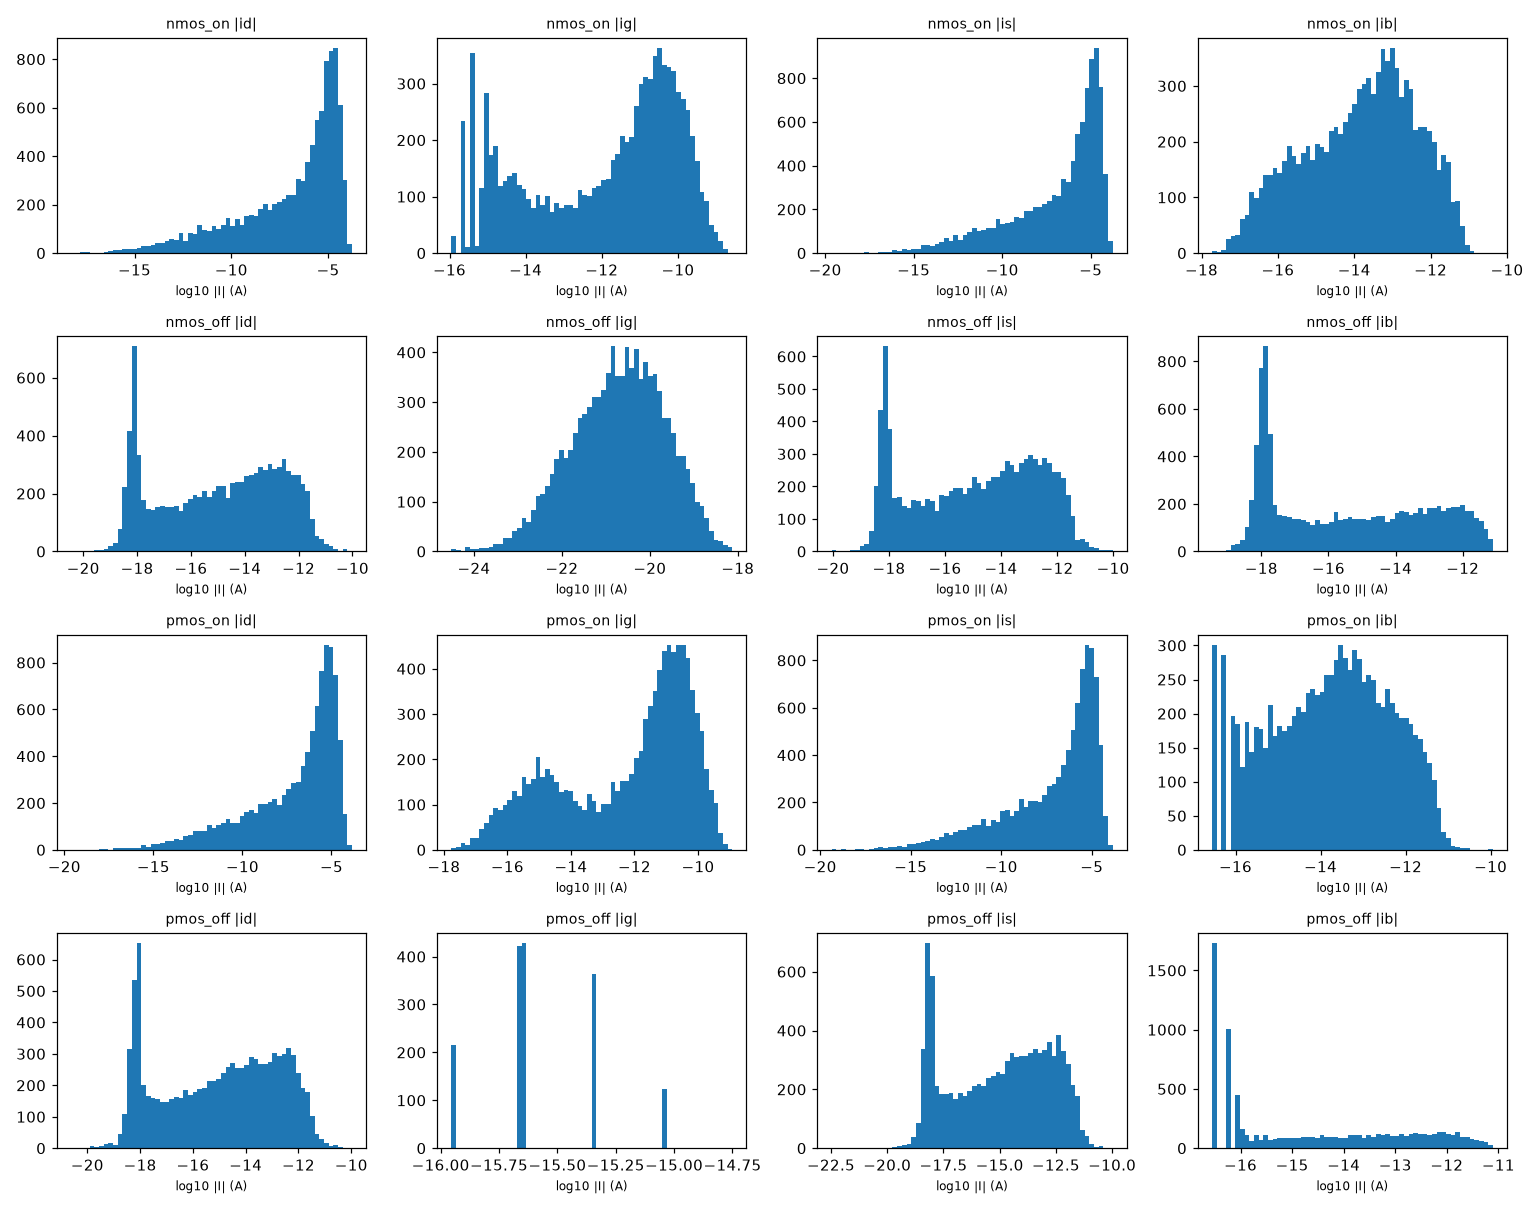
\includegraphics[width=\textwidth]{distributions.png}
\caption{Magnitude distributions of the four terminal currents for the four cases.}\label{fig:dist}\end{figure}

\paragraph{Trend plots.} Figures~\ref{fig:tT}--\ref{fig:tox} show the three required trends, obtained from controlled one-at-a-time sweeps
(all other inputs fixed). OFF current rises by a factor of about 400 between $-40$ and $125\,^\circ$C, falls by a factor of 35--46 over the $\pm10\%$
range of vth0, and the gate current falls by a factor of about 30 when toxe grows by 20\% ---all in the physically expected direction.
\begin{figure}[H]\centering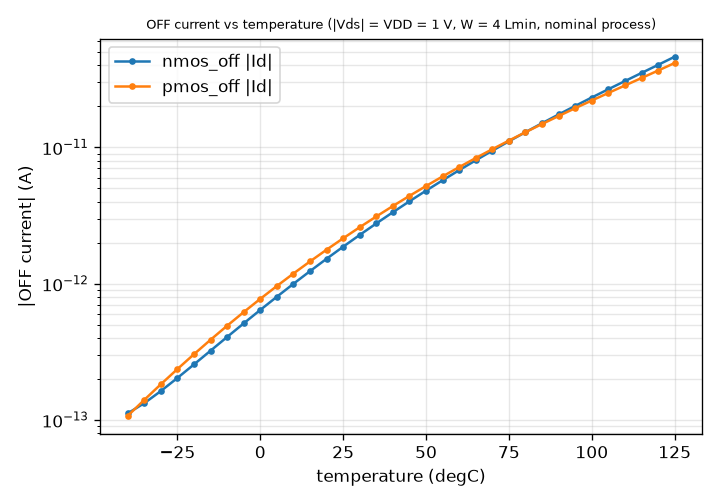
\includegraphics[width=.62\textwidth]{trend_off_vs_temperature.png}\caption{OFF current vs temperature.}\label{fig:tT}\end{figure}
\begin{figure}[H]\centering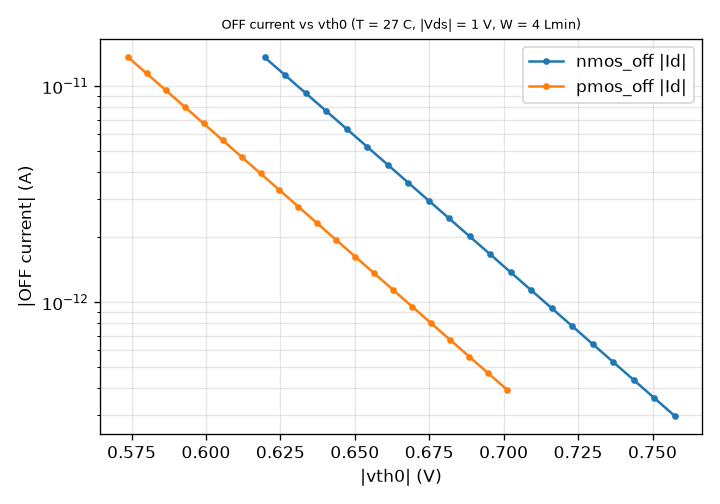
\includegraphics[width=.62\textwidth]{trend_off_vs_vth0.png}\caption{OFF current vs vth0.}\label{fig:vth}\end{figure}
\begin{figure}[H]\centering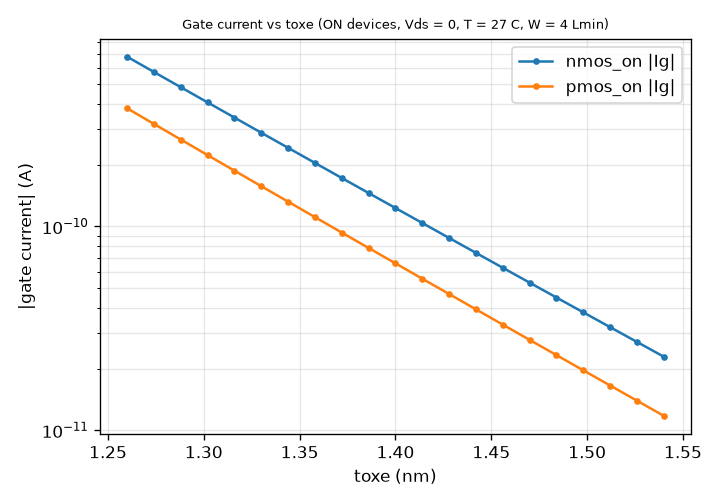
\includegraphics[width=.62\textwidth]{trend_ig_vs_toxe.png}\caption{Gate current vs toxe (ON devices, $V_{ds}=0$).}\label{fig:tox}\end{figure}
